\message{ !name(chapter0.tex)}
\message{ !name(chapter0.tex) !offset(-2) }
\chapter{The Search for Gravitational Waves}

\section{Introduction}
The field of ground-based gravitational-wave (GW) physics is rapidly
approaching a state with a high likelihood of detecting GWs for the
first time. Such a detection will not only validate part of Einstein's
general theory of relativity, but initiate an era of astrophysical
observation of the universe through GWs. Gravitational waves are
generated by non-axisymmetric acceleration of mass. A first
detection is expected to witness an event such as a supernova or
binary black hole/neutron star merger. 

\section{The theory of gravitational waves}
Gravitational radiation is a perturbation to the flat space-time
Minkowski metric 

\section{Astrophysics/cosmology motivations}

\section{Sources}
\begin{itemize}
\item inflation of the universe
\end{itemize}

\section{Methods of detection}
\begin{itemize}
\item Hulse/Taylor
\item Resonant bars
\item Pulsar timing
\item CMB polarization (B-modes)
\item Interferometry
\end{itemize}

\section{State of ground-based interferometry}
A network of first generation kilometer scale laser interferometer
gravitational-wave detectors completed its integrated 2-year data
collection run in 2007, called S5. The instruments were: the American
Laser Interferometer Gravitational-wave Observatories (LIGO)\cite{Abbott2009LIGO},
one in Livingston, LA with 4 km long arms and two in Hanford, WA with
4 km and 2 km long arms; the 3 km French-Italian detector
VIRGO\cite{Acernese2008Virgo} in Cascina, Italy; and the 1.2 km
German-British detector GEO\cite{Luck2006Status} in Ruthe, Germany. Multiple
separated detectors increase detection confidence through signal
coincidence and improve source localization through triangulation.

The first generation of LIGO, known as Initial LIGO, achieved its
design goal of sensitivity to GWs in the 40~Hz - 7000~Hz band which
included an impressive record strain sensitivity of
$2\times10^{-23}/\sqrt{\mathrm{Hz}}$ at 155~Hz. However, only the
loudest of sources produce enough GW strain to appear in LIGO's band,
and no gravitational wave has yet to be found in the S5 data. A second
generation of LIGO detectors, Advanced LIGO, has been designed to be
at least an order of magnitude more sensitive at several hundred Hz
and above and include an impressive increase in bandwidth down to
10~Hz, dramatically increasing the chances of detection. To test some
of Advanced LIGO's new technologies, an incremental upgrade to the
detectors was carried out after S5 \cite{Adhikari2006Enhanced}. This
project, Enhanced LIGO, culminated with the S6 science run from July
2009 to October 2010. Currently, construction of Advanced LIGO is
underway. VIRGO and GEO will both undergo their own upgrades as well
\cite{Acernese2008Virgo} \cite{Luck2010Upgrade}. See Figure
\ref{fig:h_all} for achieved and theoretical noise curves.

\begin{figure}
\begin{centering}
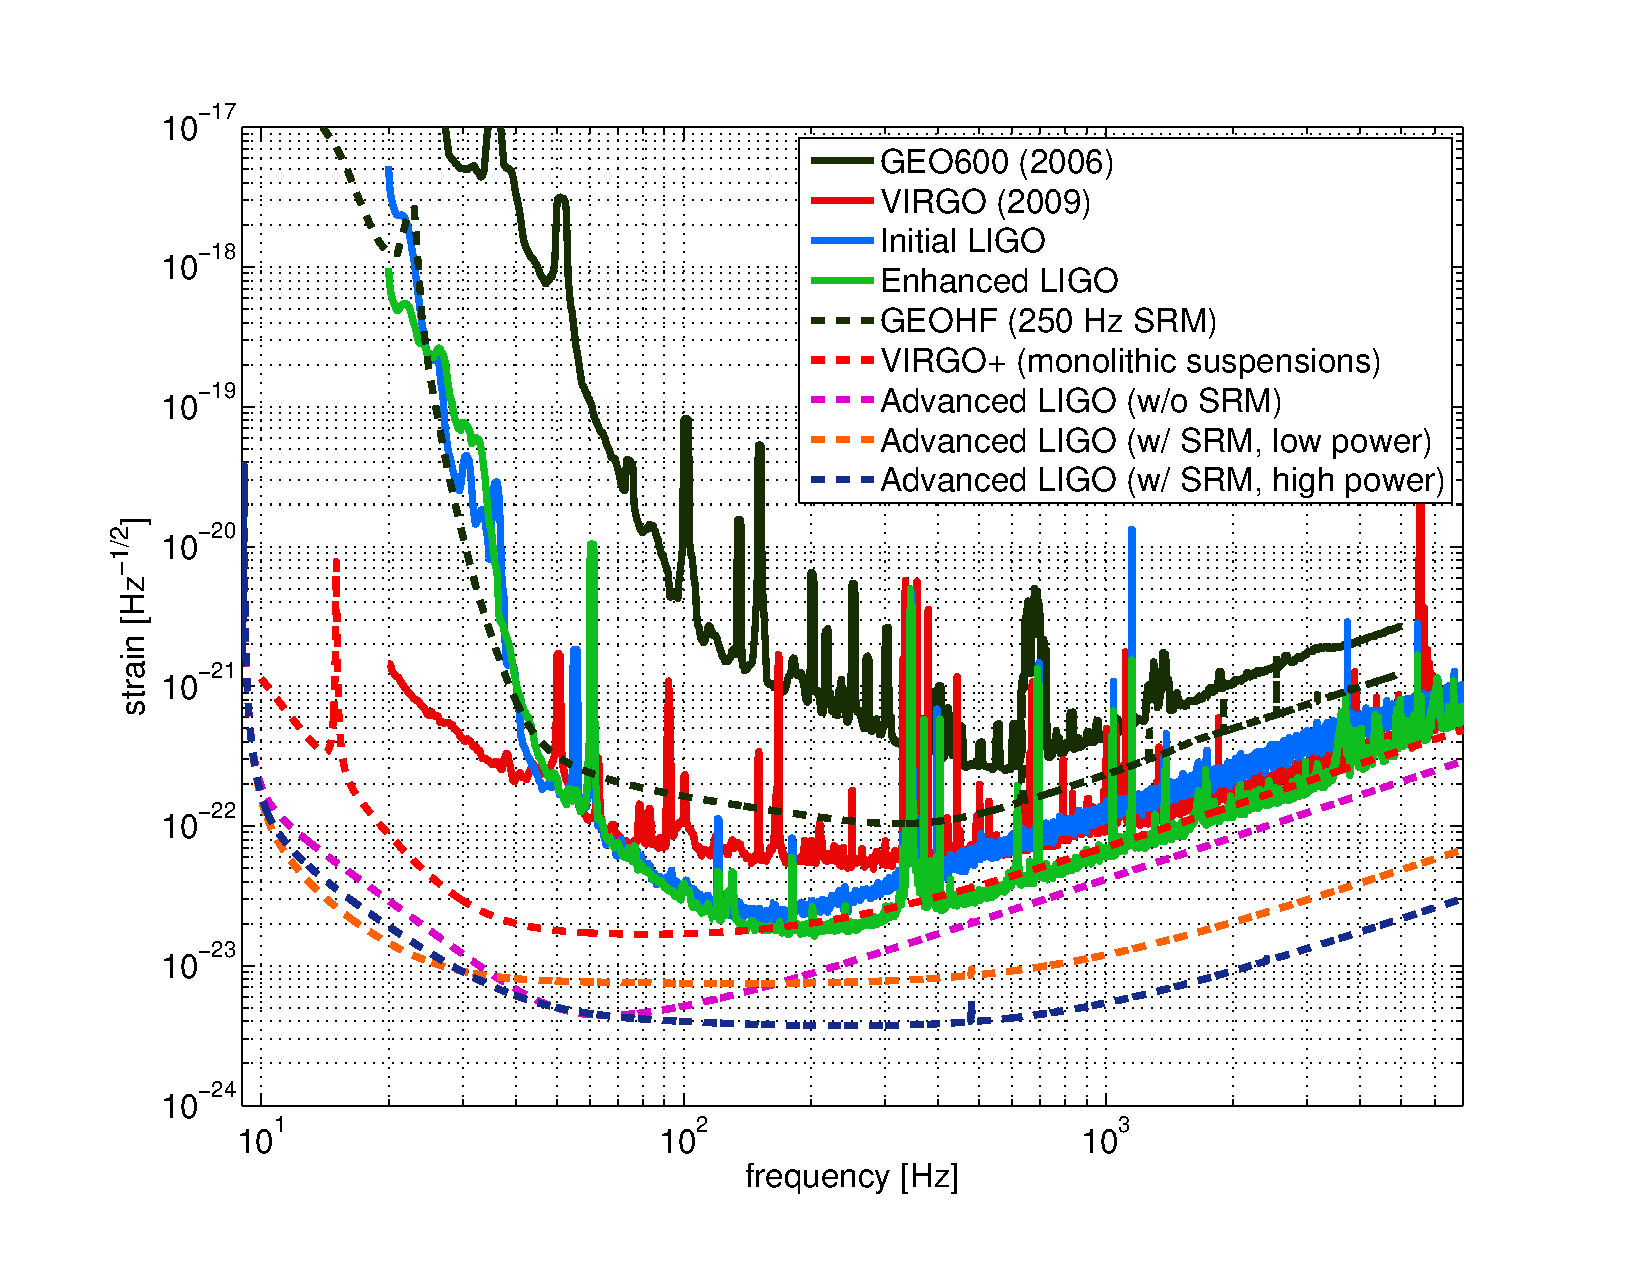
\includegraphics[width=0.7\textwidth]{figures/GWnetwork_sensitivities.pdf}
\caption{Strain sensitivities of LIGO-VIRGO collaboration interferometers.}
\label{fig:h_all}
\end{centering}
\end{figure}

The baseline Advanced LIGO design \cite{AdvLigoSysDesign} improves
upon Initial LIGO by featuring better seismic isolation, the addition
of a signal extraction mirror at the output port, homodyne readout,
and an increase in laser power from 10~W to 200~W. The substantial
increase in laser power improves the shot-noise-limited sensitivity,
but introduces a host of radiation pressure and thermally induced side
effects that must be addressed for proper operation.

The recently completed Enhanced LIGO tested portions of the Advanced
LIGO designs so unforeseen difficulties could be addressed and so that
a more sensitive data taking run could take place. An output mode
cleaner was designed, built and installed, and DC readout of the GW
signal was implemented \cite{Fricke2011DC}. An Advanced LIGO active
seismic isolation table was also built, installed, and tested
\cite{KisselThesis}. In addition, the 10~W Initial LIGO laser was
replaced with a 35~W laser \cite{Frede2007Fundamental}. Accompanying
the increase in laser power, both the Alignment Sensing and Control
and Input Optics were modified. The upgrades of these two subsystems
make up the content of this dissertation. 


\message{ !name(chapter0.tex) !offset(-94) }
